\documentclass[11pt]{article}
\usepackage[utf8]{inputenc}
\usepackage{graphicx}
\usepackage{hyperref}
\usepackage[a4paper, total={6in, 8in}]{geometry}

\title{Notes on Chapter 9 - A Simplistic Introduction to Algorithmic Complexity}
\author{Swarup Tripathy \thanks{John V Guttag}}
\date{May 2022}


\begin{document}
    \maketitle
    A curated list of important points for my reference.\\
    \begin{enumerate}
        \item Exhaustive enumeration was so slow as to be impractical for many combinations of x and epsilon. 
        For example, evaluating \textit{squarerootExhaustive(100,0.0001)} requires roughly one billion iterations of the while loop.
        In contrast, evaluating \textit{squarerootBi(100,0.001)} takes roughly twenty iterations of a slightly more complex while loop.
        \item Asymptotic Notation describes the Complexity of an algorithm as the size of its inputs approaches Infinity.
        \item Following rules of thumb in describing the asymptotic Complexity of an algorithm
        \begin{itemize}
            \item If the running time is the sum of multiple terms, keep the one with the larges growth rate, and drop the others
            \item If the remaining term is a product, drop any constants.
        \end{itemize}
        \item \textbf{Big O Notation}
        \begin{itemize}
            \item So, the story begins in 2009 in a region of south africa when there was a slow internet issue in the office.
            \item They wanted to test how much time will it take for the internet to send a chunk of data to another office located 50 miles away as compared to a bird carrying that chunk of data.
            \item The Bird won, and it went all over the press that the bird was faster than the internet but this was something of a ridiculous experiment.
            \item Everything depends upon the chunk of data as in for the bird this would remain the same while for the internet this would be something of an additional load. It's not going to take longer for the bird since the usb stick carries more data.
            \item So of course for a sufficiently large file the pigeon's going to win.
            \item We define the pigeon transfer speed as \textit{O(1)} $\rightarrow$ it's constant time wrt the size of the input. It doesn't take any longer with more input.
            \item Whereas the Internet Transfer time is \textit{O(n)} $\rightarrow$ it scales linearly with respect to the amount of input. Twice amount of data will take roughly twice the amount of time.
            \item BIG O $\rightarrow$ How time scales with respect to some input variables.
            \begin{center}
                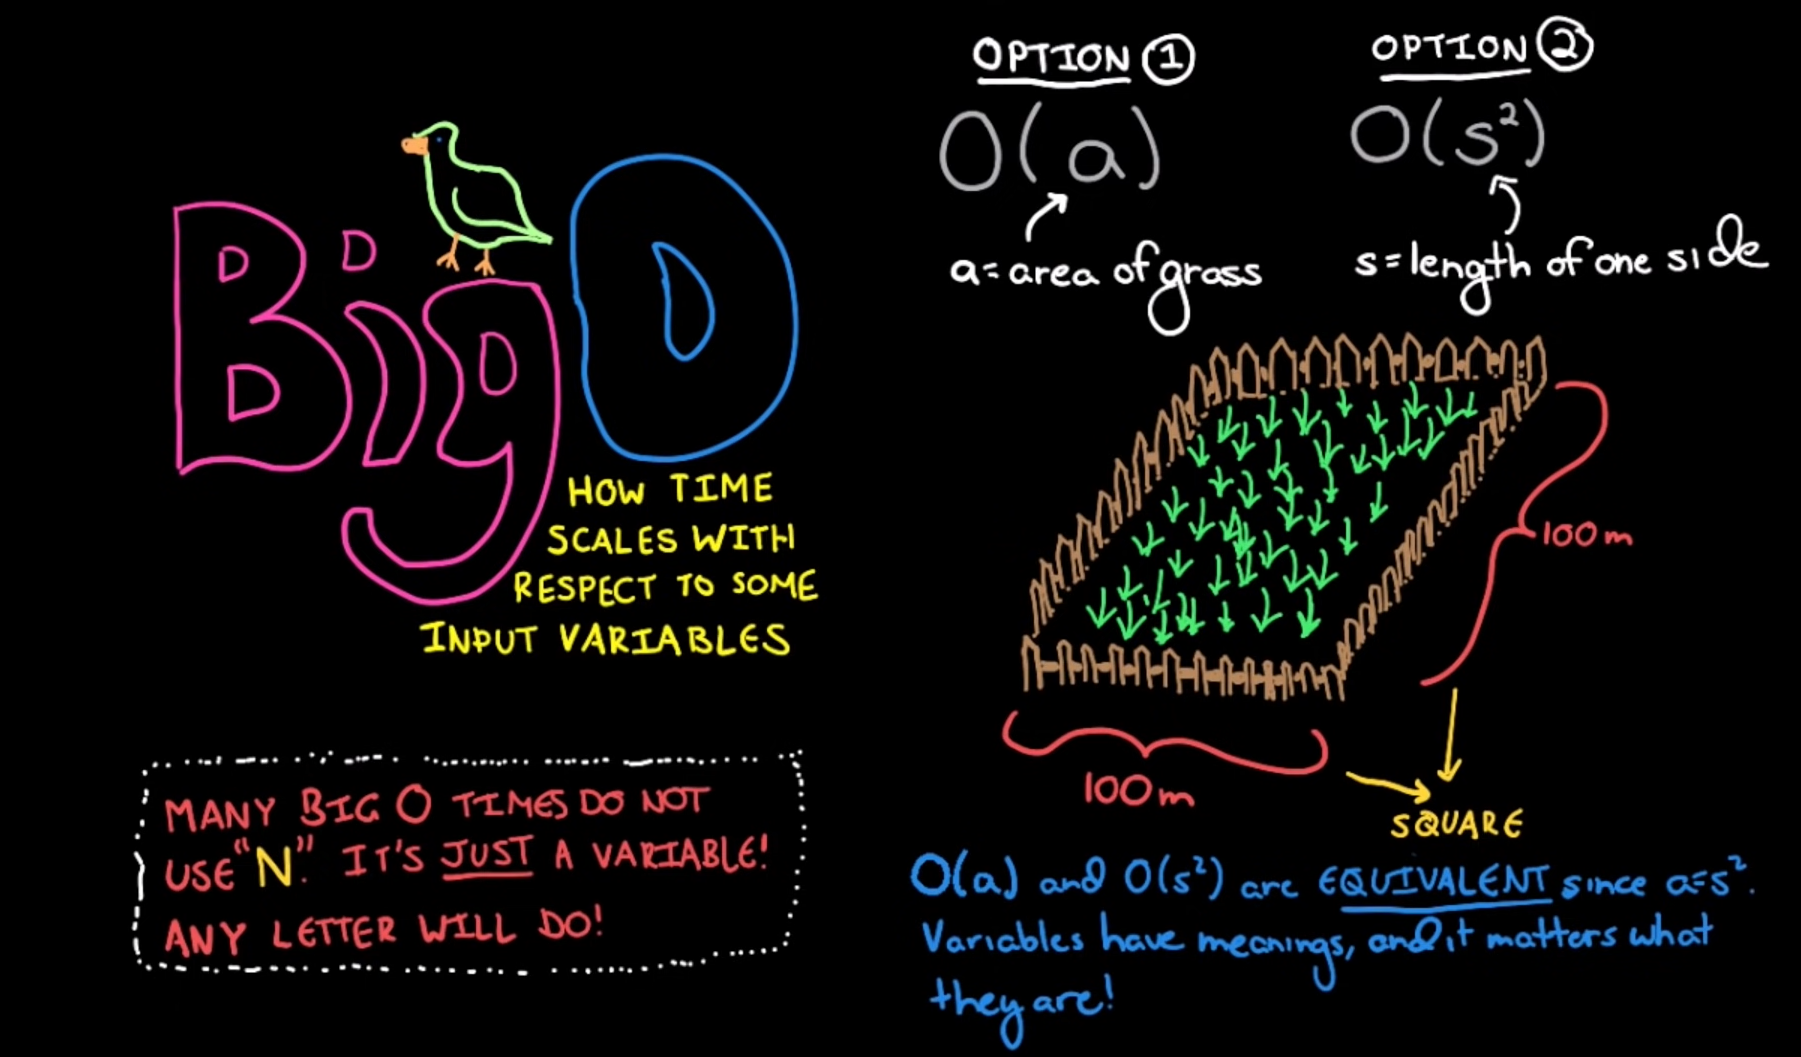
\includegraphics[width=13cm]{imgs/bigO.png}
                \textit{How much time does it take to mow the grass off the field.}
            \end{center}
            \item Important rules of Big O
            \begin{itemize}
                \item Different Steps get added
                \begin{verbatim}
            function something(){
                doStep1(); // O(a)
                doStep2(); // O(b)
            }
    // after adding their runtime it becomes O(a+b)
                \end{verbatim}
                \item Drop Constants
                \begin{verbatim}
            function minMax1(array){
                min,max = NULL
                for each e in array
                    min = MIN(e,min)
                for each e in array
                    max = MAX(e,max)
            }
    // Above: individual runtime O(n) and O(n) and 
    // as a whole remains O(n) and not O(2n) <= drop the constant 2.

            function minMax1(array){
                min,max = NULL
                for each e in array
                    min = MIN(e,min)
                    max = MAX(e,max)
            }
    // Above: runtime altogether is O(n)
                \end{verbatim}
                \item Different inputs $\rightarrow$ Different Variables
                \begin{verbatim}
            int intersectionSetSize(arrayA, arrayB){
                int count=0;
                for a in arrayA{
                    for b in arrayB{
                        if a==b{
                            count = count + 1
                        }
                    }
                }
                return count
            }
    // Above: runtime is not O(n^2) rather it will be O(a.b)
                \end{verbatim}
                \item Drop non-dominate terms
                \begin{verbatim}
            function example(arrray){
                max=NULL
                for each a in array{
                    max = MAX(a,max)
                }
                print max
                for each a in array{
                    for each b in array{
                        print a,b
                    }
                }
            }
// Above: here runtime as discusses before could be O(n+n^2) but 
// here n^2 dominates so we neglect n and 
// final Big O notation will be O(n^2)
                \end{verbatim}
            \end{itemize}
        \end{itemize}
    \end{enumerate}
\end{document}